\documentclass[11pt,a4paper]{article}
\usepackage[utf8]{inputenc}
\usepackage[english]{babel}
\usepackage{amsmath}
\usepackage{amsfonts}
\usepackage{amssymb}
\usepackage{graphicx}
\usepackage{todonotes}
\usepackage[left=2cm,right=2cm,top=2cm,bottom=2cm]{geometry}
\usepackage{caption}
\usepackage{subcaption}

\begin{document}
%%%%%%%%%%%%%%%%%%%%%%%%%%%%%%%%%%%%%%%%%%%%%%%%%%%%%%%%%%%%%%%%%%%%%%%%%%%%%%%
%\vspace*{\stretch{1.0}}
\begin{center}
\Large\textbf{Report 4: Unsupervised learning: PCA and SOM}\\
\large Author: \textit{Jannes Nys}
\end{center}
%\vspace*{\stretch{2.0}}
%%%%%%%%%%%%%%%%%%%%%%%%%%%%%%%%%%%%%%%%%%%%%%%%%%%%%%%%%%%%%%%%%%%%%%%%%%%%%%%


\section{Principal Component Analysis on Handwritten Digits}
In the Principle Component Analysis, one decomposes the data entries into the principal eigenvectors of the covariance matrix. Each figure is then approximated by a linear combination (for linear PCA) of the limited set of eigenvectors.

Figure~\ref{fig:recon_and_cumsum} shows the total reconstruction error as a function of the number of eigenvectors used in the PCA projection. Figure~\ref{fig:recon_and_cumsum} also shows the total reconstruction error. These figures illustrate that both are proportional. Hence, by setting the required maximum reconstruction error, one can choose a proper number of eigenvectors of the covariance matrix to span the compressed space based on the cumulative sum of the eigenvalues.

When $k$ is equal to $256$, which is the dimension of the original basis, the eigenbasis of the PCA spans the full space of the original figures. Hence, the reconstruction error is approximately\footnote{Due to computational round-off errors, during the eigenvector decomposition and reconstruction, the obtained is not exactly $0$, but rather $6.7150 \times 10^{-29}$.} zero, since the PCA is now a rotation of the figures, which is inverted exactly upon reconstruction.

As an example, we show a reconstructed image for a number of dimensions of the PCA basis in Fig.~\ref{fig:reconstruction_example}. As the basis increases, the reconstructed image converges towards the original image.

\begin{figure}[htb]
\centering
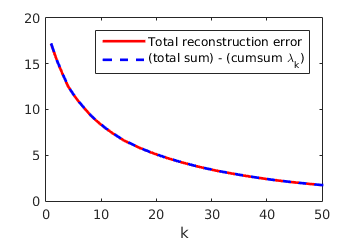
\includegraphics[width=0.4\textwidth]{figs/recon_and_cumsum.png}
\caption{Total sum of all eigenvalues minus the cumulative sum of the reconstruction $k$ largest eigenvalues of the covariance matrix (dashed blue) and mean-squared reconstruction error (solid red) as a function of the dimensionality of the PC basis.\label{fig:recon_and_cumsum}}
\end{figure}

%\begin{figure}[htb]
%\centering
%\subcaptionbox{Total sum of all eigenvalues minus the cumulative sum of the reconstruction $k$ largest eigenvalues of the covariance matrix\label{fig:cumsum}}{
%\centering
%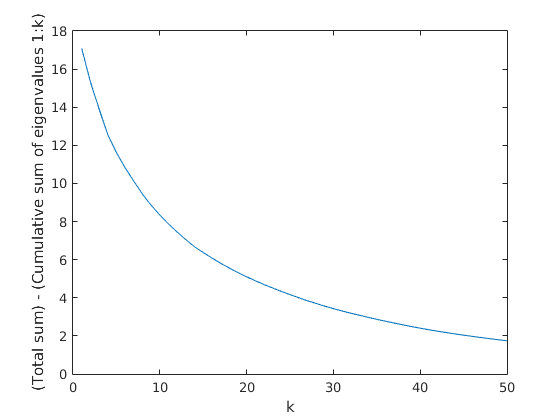
\includegraphics[width=0.48\columnwidth]{figs/cumsum.png}
%}
%\subcaptionbox{Total squared reconstruction error as a function of the dimensionality of the projection basis.\label{fig:total_recon_error}}{
%\centering
%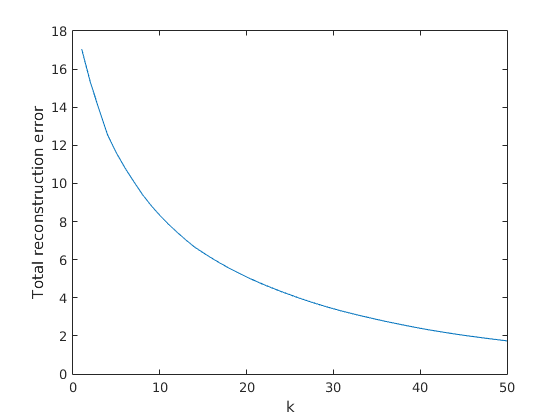
\includegraphics[width=0.48\columnwidth]{figs/total_recon_error.png}
%}
%\end{figure}

\begin{figure}[htb]
\centering
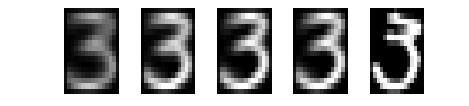
\includegraphics[width=\textwidth]{figs/reconstruction_steps.png}
\caption{Example of a reconstruction of an image using a basis of (f.l.t.r.) $1,2,3$ and $4$ principal eigenvectors. The outer-rightmost figure is the original, uncompressed image. It was observed that for this data item, a basis of $\sim 50$ eigenvectors is required to restore the image properly.\label{fig:reconstruction_example}}
\end{figure}

\section{Self-organizing maps: concentric cylinders}


\section{Self-organizing maps: unsupervised clustering of the Iris data set}


\end{document}